\chapter[Introducción]{Introducción}
\thispagestyle{empty}

\clearpage
\newpage
\thispagestyle{empty}
\mbox{}
\newpage


El calentamiento global es el mayor problema ambiental que enfrenta el mundo, el 
mismo se refiere al efecto que producen las actividades humanas en el clima, como 
la quema de combustibles fósiles o la deforestación, que emiten a la atmósfera
grandes cantidades de dióxido de carbono, CO$_2$, entre otros gases de efecto 
invernadero. Estos gases absorben la radiación infrarroja emitida por la tierra 
provocando un incremento de la temperatura de la misma que lleva asociado un 
aumento en la frecuencia y la intensidad de eventos climáticos extremos 
~\cite{houghton2005}. Según el Panel Intergubernamental del Cambio Climático 
(IPCC), desde la época preindustrial, las actividades humanas han provocado 
aproximadamente 1.0$^{\circ}$C de calentamiento global y al ritmo actual se van 
a sobrepasar los 1.5$^{\circ}$C antes del 2050, un cambio en la temperatura
media que las emisiones previas por sí solas no habían alcanzado
~\cite{harvey2018}. Limitar el calentamiento a esta temperatura requiere que se 
realicen rápidamente cambios sin precedentes en la tecnología y en el 
comportamiento humano. Uno de los cambios más importante es el de la matriz 
energética, en la cual las energías renovables deberán suministrar alrededor del 
80\% de la energía para 2050, donde los vectores energéticos, como las baterías 
de litio, juegan un rol fundamental debido a la intermitencia de estas formas de 
generación de energía.

El litio es el metal más liviano de la tabla periódica y uno de los elementos más
importantes dentro de los minerales necesarios en la producción de baterías de
litio. En particular, para la Argentina tiene un interés económico, social, 
industrial y tecnológico ya que es uno de los países que integran, junto a 
Bolivia y Chile, el Triangulo de Litio, el cual acumula el 70\% de las reservas 
mundiales de este mineral. Aún más importante que esta cantidad de reservas es 
que las mismas se encuentran en salares que, a grandes rasgos, es más barato
extraer litio de ellos en comparación a las pegmatitas, heroctitas o jadaritas, 
que son las rocas de las cuales se puede extraer litio en una minería usual.
A pesar de esto se tienen que llevar a cabo distintas consideraciones ambientales,
sociales y legales del proceso de extracción e incentivar el desarrollo de valor
agregado a dicha extracción ~\cite{heredia2020}.

En esta tesis se presentan estudios realizados mediante el uso de simulaciones 
computacionales en... TODO


\section{Transición energética}

La demanda internacional de energía sigue en aumento debido al crecimiento 
poblacional rápido y a los avances en la civilización, más del 80\% de la misma
sigue siendo producida por combustibles fósiles, que son limitados en recursos 
y tienen un impacto grave en el medio ambiente. Sin políticas comprometidas con 
la transición energética no se espera que esta proporción disminuya, dejando 
lugar a la producción de energía mediante fuentes renovables, en los próximos 20
años. Si el cambio en la matriz energética se deja en manos del mercado, las 
fuentes de energía limpias no sustituirán por sí solas a los métodos tradicionales
hasta que no sólo alcancen una paridad de precios, si no que se vuelvan 
considerablemente más baratas de manera que justifiquen dicho cambio
~\cite{davidson2019}. Dicho esto, cumplir los objetivos climáticos y realizar la 
transición hacia un futuro con menos carbono va a requerir inversiones 
sustanciales por parte de los gobiernos ~\cite{leonhardt2022}.

La gran mayoría de las naciones desarrolladas han implementado un marco legal de 
apoyo y habilitación para ayudar a promover la integración de las energías 
renovables modernas en sus sistemas energéticos. Estas políticas se han 
desarrollado como resultado, o en apoyo, de acuerdos internacionales como el 
Acuerdo de París, el Protocolo de Kioto o el Green Deal europeo. Los objetivos 
de las energías renovables y los incentivos fiscales dirigidos al sector 
energético son las dos políticas más comunes en países en desarrollo para apoyar 
la transición energética ~\cite{cantarero2020}.

En Argentina el sector energético depende altamente de la utilización de 
combustibles fósiles, donde la capacidad de generación de energía está 
principalmente atada a las centrales térmicas convencionales y a grandes 
centrales hidroeléctricas, mientras que tan sólo una pequeña cantidad proviene 
de plantas nucleares y de fuentes de energías renovables. En cuanto al potencial
de producción de energía de fuentes renovables, Argentina tiene una gran 
capacidad eólica y solar. El gobierno nacional viene incentivando la instalación 
de dichas fuentes de energía desde 2009, mediante el programa GENREN. A fines 
del 2015 se estableció un objetivo de que el 20\% de la energía fuera generada
mediante estas fuentes para 2025 y en 2016 se introdujo un nuevo esquema de 
compra con el programa RenovAr ~\cite{schaube2018}. Este desarrollo viene 
acompañado de un amplio espectro de investigaciones académicas 
interdisciplinarias.

\subsection{Energías renovables}

Existen muchas formas de generación de energías renovables, entre ellas destacan:
\begin{itemize}
    \item la \textbf{biomasa}, que permite obtener la energía química 
        que se encuentra almacenada en la materia orgánica mediante la quema de 
        la misma,
    \item la \textbf{hidráulica}, que aprovecha la energía cinética y potencial
        de la corriente del agua, la \textbf{marina}, transportada en las olas
        del mar,
    \item la \textbf{eólica}, obtenida a partir de la energía cinética del viento,
    \item la \textbf{solar}, que permite producir energía a partir de la radiación
        electromagnética del sol.
\end{itemize}
La producción de dispositivos eficientes de obtención de energía renovable es un 
requisito esencial para mejorar la eficiencia y, finalmente, reducir el costo de 
las fuentes de energía renovables. Este es uno de los retos a los que se 
enfrenta el establecimiento generalizado de las mismas en comparación con fuentes
de energía tradicionales ~\cite{olabi2022}. Para dar un ejemplo, la energía solar 
se encuentra disponible en todas partes y ya se aplica comercialmente en varios 
sectores. Uno de los principales retos a los que se enfrenta la misma es a los 
días nublados, que afecta negativamente a la producción de energía. La 
generalización de los sistemas solares fotovoltaicos requiere sistemas eficientes 
de almacenamiento de energía, donde las baterías son las más accesibles. 

\subsection{Sistemas de almacenamiento y transporte de energía}

Como una solución al problema de la alta intermitencia, la baja predictibilidad 
diaria y la variación estacional de energías renovables, se introducen sistemas 
de almacenamiento de energía. La energía de estas fuentes debe ser almacenada 
cuando están produciendo energía por demás y esta puede ser liberada cuando se 
requiera. Dichos sistemas pueden ser clasificados a grandes rasgos en mecánicos, 
electroquímicos, químicos o térmicos ~\cite{khan2019}.

En el caso de los sistemas de almacenamiento de energía mecánicos, la energía se
almacena realizando algún trabajo mecánico, entre ellos se encuentra, por ejemplo,
el aire comprimido. En el almacenamiento de energía térmica se utiliza la energía 
térmica que se produce al calentar o enfriar un medio.

En el sistema químico, la energía se almacena en forma de energía química 
almacenada en distintos materiales. Se tienen principalmente dos tipos, los
biocombustibles o el hidrógeno. En este último caso, la energía eléctrica se 
utiliza para descomponer el agua en oxígeno e hidrógeno, estos gases se almacenan 
y se transportan para luego volver a combinarse y liberar la energía almacenada.

Por último, dentro de los sistemas de almacenamiento de energía electroquímicos 
se encuentran las baterías y los capacitores. En las baterías, tanto a la entrada 
como la salida de energía la misma se encuentra en forma de energía eléctrica 
mientras que la electricidad se almacena en energía química. 


\section{Baterías}

Las baterías pueden ser clasificadas dentro de dos grupos, primarias o 
secundarias. Las baterías primarias no son recargables, es decir que solo pueden
ser utilizadas hasta que su energía se agota, esto se debe a que sus reacciones
químicas no suelen ser reversibles. Por otro lado, las baterías secundarias son 
aquellas que se pueden recargar, es decir que pueden ser reutilizadas muchas 
veces, sus reacciones químicas son reversibles y puede volver a obtenerse los 
reactantes si se le aplica una corriente eléctrica a la celda.

La primera batería concebida fue inventada por Alessandro Volta en 1800 para 
estudiar los descubrimientos de Luigi Galvani, la misma basa su funcionamiento 
en la combinación de zinc con cobre y se la conoce como pila voltaica, fue 
crucial para los primeros experimentos electroquímicos. En 1866 la celda primaria 
de Leclanche, predecesora de la pila de zinc-carbono actual, se convirtió en una
de las primeras baterías comerciales al ser utilizada en estaciones de telegrafía
y en los primeros teléfonos. A mediados del siglo XIX surgió la necesidad de un 
sistema de almacenamiento recargable debido a la invención del generador 
eléctrico, la misma fue satisfecha por Gaston Panté al presentar la batería de 
plomo-ácido. Durante este último periodo de tiempo y principios del siglo XX, 
los motores de combustión interna y los motores eléctricos compitieron como medios
de propulsión en los automóviles. Con el descubrimiento de reservas de petróleo 
mayores a principios del siglo XX y el desarrollo de automóviles de gasolina más
cómodos, los vehículos eléctricos se vieron rápidamente superados por los de 
motores de combustión interna y se dejaron de fabricar. Por desgracia, el sector 
del transporte se convirtió en uno de los responsables de gran parte de la 
contaminación.

Un siglo después aparecieron nuevas iniciativas en el campo de las baterías con
el desarrollo del consumo de la electrónica portátil, que requiere una batería 
recargable de alta densidad energética que no es una condición que cumpla la 
batería de plomo-ácido. Inicialmente se prestó mucha atención al sistema 
níquel-cadmio hasta ser superado por las baterías de iones de litio (LIB) a 
principios de la década del 1990. Desde esa fecha, las LIB continúan mejorando
constantemente y prometen desempeñar un papel vital en el desarrollo de vehículos
eléctricos y el almacenamiento de energía de fuentes alternativas. % schipper2016

En la figura \ref{fig:densidad} puede observarse como se posicionan las distintas
baterías de litio actuales y las que se encuentran en etapa de investigación
en comparación a baterías anteriores. Puede notarse que cada vez se está buscando
utilizar baterías más chicas y más livianas.
\begin{figure}
    \centering
    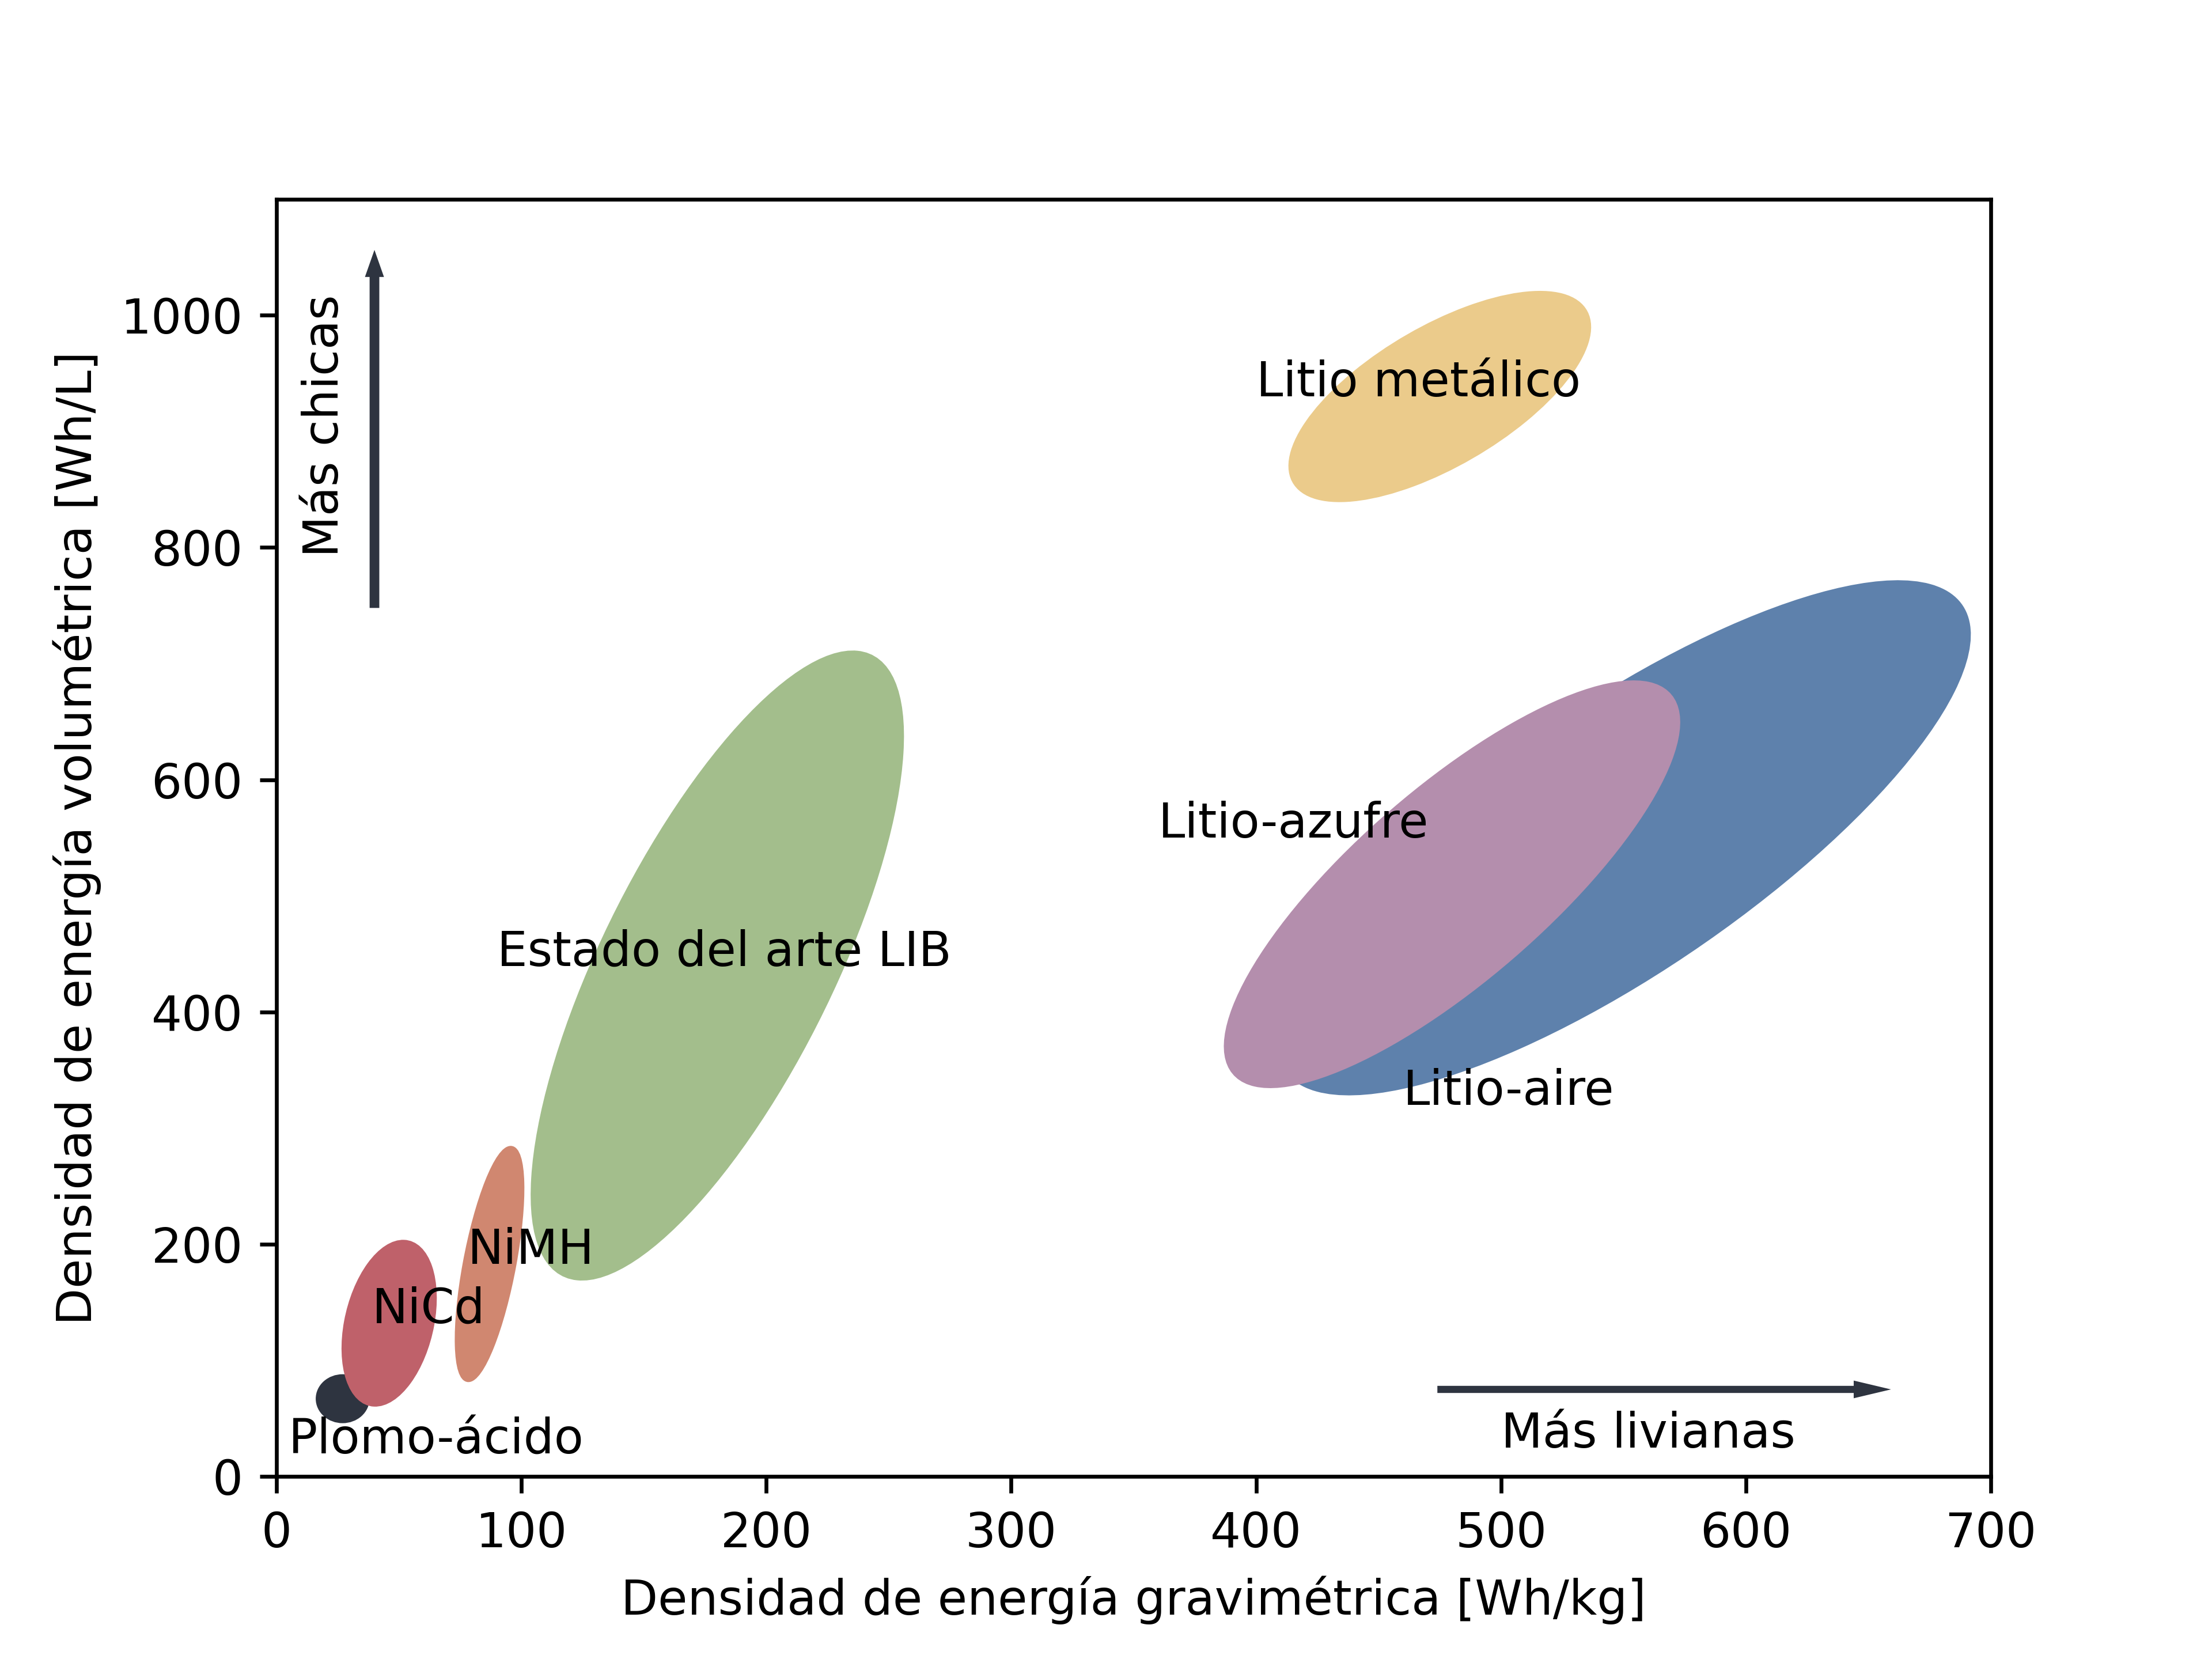
\includegraphics[width=0.8\textwidth]{introduccion/densidad_de_energia.png}
    \caption{Densidad de energía por unidad de volumen y por unidad de masa para 
    distintas baterias ~\cite{tarascon2011, placke2017}.}
    \label{fig:densidad}
\end{figure}

TODO: Funcionamiento de una batería, sus partes. 

\subsection{Baterías de ion litio}

Las baterías de litio son dispositivos electroquímicos ampliamente utilizados 
como fuentes de energía. Entre las propiedades físicas del litio destacan su 
peso molecular bajo (7 g mol$^{-1}$), su densidad baja (0.534 cm$^3$), su 
capacidad específica alta (3860 mAh g$^{-1}$) y su potencial de reducción bajo 
(-3.04 V vs. SHE), estas propiedades lo convirtieron en un material que puede 
ser utilizado como ánodo para baterías. 

A finales de la década del 1950 se observó que el litio metálico formaba una capa 
de pasivación, llamada interfaz de electrolito sólido (SEI, de sus siglás en 
inglés, \textit{solid electrolyte interface}), con distintos electrolitos 
no-acuosos permitiendo prevenir una reacción química directa entre estas dos 
componentes, pero dejando que los iones de litio la atraviesen ~\cite{peled1979}. 
Esto generó un interés que llevó a la fabricación de baterías primarias de litio 
en la década del 1960 utilizando distintos tipos de cátodos incluyendo dióxido de 
sulfuro de litio (LiSO$_2$), óxido de manganeso de litio (LiMnO$_2$) y óxido de 
cobre de litio (LiCuO), entre otros. Desafortunadamente, la formación de la SEI 
no es estable durante ciclos prolongados y se agrieta, lo que lleva a un consumo 
continuo de electrolito y litio para la reformación continua de la SEI 
~\cite{besenhard1976}. Y lo que es aún peor, la deposición desigual de litio en 
la SEI agrietada conduce al crecimiento de dendritas de litio, que terminan 
rompiéndose y formando islas de tamaño nanométrico de litio altamente reactivo, 
lo que reduce la estabilidad térmica de la celda ~\cite{yamaki1998}. Las 
dendritas también pueden crecer lo suficiente como para generar un contacto 
entre el ánodo y el cátodo, provocando un cortocircuito. 

Avances posteriores en la comprensión de la intercalación de litio en diferentes
materiales dio origen a las baterías recargables de ion-litio. El primero de 
estos materiales fue utilizado por EXXON para una primera versión de las mismas.
Whittingham demostró en 1976 que el litio se intercala entre las capas que se 
forman en los metales de transición en una proporción de un mol que provoca una
expansión del parámetro de red ~\cite{whittingham1976}. El material más 
interesante de estos era el TiS$_2$, que ofrece el menor peso molecular, un costo 
potencialmente bajo y es un conductor eléctrico. Sin embargo, esta batería seguía
utilizando litio metálico como ánodo, presentando los problemas ya mencionados. 

La necesidad de un material catódico de intercalación de litio de alto voltaje 
que se presentaba en la época fue resuelta por el compuesto laminar LiCoO$_2$ 
(LCO) que fue desarrollado por el grupo de investigación de Goodenough en 1980
~\cite{mizushima1980}. La gran diferencia de tamaño entre el cobalto y el litio 
da lugar a un material de capas perfecto con poca o ninguna mezcla de cationes. 
Este aspecto hace que la síntesis estequiométrica de LCO y de fase pura sea muy 
fácil en diversas condiciones. 

Sin embargo, se necesitaba un material anódico estable que permitiera intercalar
los iones de litio. No fue hasta el 1990 que esto se cumplió, año en el que el
grupo de investigación de Dahn descubrió dicha estabilidad en los ánodos de 
grafito en soluciones electrolíticas no acuosas al estudiar la intercalación de 
forma reversible en los primeros 19 ciclos utilizando como electrolito una mezcla 
de disolvente de carbonato de propileno y carbonato de etileno ~\cite{fong1990}. 
Esto se da gracias a la formación de una SEI estable durante el primer ciclo de 
intercalación. 

En la tabla \ref{t:historia} se presentan las primeras baterías secundarias de 
litio comercializadas hasta 1991, año en el que se dejó de utilizar litio 
metálico como ánodo y se comenzó a utilizar uno de grafito. En la misma puede 
notarse el avance con los años de la densidad de energía, sin embargo este no es 
el único parámetro a tener en cuenta en el progreso ya que también tienen que 
considerarse la cantidad de ciclos que se pueden realizar, el tiempo de carga, la 
razón de descarga y el precio de producción ~\cite{reddy2020}. 
\begin{table}[h]
    \centering
    \caption{Primeras baterías de litio recargables comercializadas 
    ~\cite{reddy2020}.}
    \setlength\extrarowheight{2pt}\stackon{%
    \begin{tabular}{c c c c}
        \toprule
        \thead{\normalsize\bfseries Sistema\\\normalsize\bfseries electroquímico} & 
        \thead{\normalsize\bfseries Voltaje (V)} & 
        \thead{\normalsize\bfseries Densidad de energía\\\normalsize\bfseries específica (Wh/kg)} & 
        \thead{\normalsize\bfseries Compañía comercial} \\
        \midrule
        Li||TiS$_2$ & 2.1 & 130 & Exxon (1978) \\
        Li||LiAlCl$_4$-SO$_2$ & 3.2 & 63 & Duracell (1981) \\
        Li||NbSe$_3$ & 2.0 & 95 & Bell Telephone Lab. Inc. (1983) \\
        LiAl||polianilina & 3.0 & -- & Bridgestone (1987) \\
        Li||MoS$_2$ & 1.8 & 52 & MoLi Energy (1987) \\
        Li||V$_2$O$_5$ & 1.5 & 10 & Toshiba (1989) \\
        LiAl||polipirrol & 3.0 & -- & Kanebo (1989) \\
        Li||Li$_{0.3}$MnO$_2$ & 3.0 & 50 & Tadiran (1989) \\
        LiVO$_x$ & 3.2 & 200 & Hydro-Québec (1990) \\
        C||LiCoO$_2$ & 3.6 & 150--190 & Sony (1991) \\
        \bottomrule
    \end{tabular}
    }{}
    \label{t:historia}
\end{table}

La batería que funciona mediante un cátodo de LCO, un ánodo de grafito y una
solución electrolítica no acuosa basada en LiPF$_6$ fue comercializada
exitosamente por Sony en 1991. Desde entonces las baterías de ion litio fueron
adaptadas para su utilización en dispositivos móviles, esto se debió a la
densidad de energía volumétrica alta, de alrededor de los 200 W h L$^{-1}$, que
era el doble que la de níquel-cadmio, su principal competidor en esa época.

En las últimas dos décadas se ha logrado duplicar la densidad de energía 
volumétrica de entonces, lo cual fue realizado en mayor medida gracias a una 
mejor ingeniería en la celda. El próximo desafío en el área de estudio viene 
dado en el desarrollo de LIBs que sean adecuadas para los vehículos eléctricos. 
Para lograr esto es necesario una mejora de la funcionalidad de cada una de las
partes de la batería.

Aunque el LCO supera a otros cátodos de intercalación de litio términos de 
densidad de energía volumétrica, la baja capacidad de 135 mAh g$^{-1}$ da una baja
densidad de energía gravimétrica. Para solucionar este problema se han 
comercializado, o están siendo considerados, distintos cátodos. Como una 
alternativa más barata al LCO se estudió el LiNiO$_2$, que es isoestructural al 
LCO pero posee una capacidad teórica mayor, de 273 mAh g$^{-1}$. Sin embargo,
es difícil de sintetizar y se ha observado la formación de una fase 
electroquímicamente inactiva cuando la concentración de litio alcanza el 50\% 
~\cite{ohzuku1993}. Otra de las variantes propuestas al LCO fue el compuesto 
laminar LiMnO$_2$, pero su capacidad de carga inicial de unos 220 mAh g$^{-1}$ 
desciende a 130 mAh g$^{-1}$ en los ciclos siguientes. Además se produce un 
reordenamiento bastante significativo en el que el material activo se transforma 
en la espinela LiMn$_2$O$_4$ (LMO) tras sólo 5 ciclos ~\cite{shao1999, shin2004}.
Ambos materiales son llamativos debido al bajo costo y la menor toxicidad del 
manganeso con respecto al cobalto o al níquel. Finalmente, con respecto a estos 
tres metales de transición, se desarrollaron compuestos de intercalación basados
en los mismos con la fórmula general Li(Ni$_{1-x-y}$Co$_x$Mn$_y$)O$_2$ (NCM o NMC)
~\cite{liu1999}. Para conseguir un material catódico viable, deben ser controladas
las proporciones de cada uno de los metales según los aspectos que se deseen de 
alta capacidad (más níquel), mejor estabilidad de ciclado (más cobalto) o 
seguridad/costo (más manganeso). Otra de las opciones es el dopaje con cationes
de cobalto y aluminio de LiNiO$_2$, Li(Ni$_{1-x-y}$Co$_x$Al$_y$)O$_2$ (NCA),
que en la composición Li(Ni$_{0.8}$Co$_{0.15}$Al$_{0.05}$)O$_2$ ~\cite{chen2004}
es comercializada por Panasonic y utilizado en algunos de los modelos de autos 
eléctricos de Tesla. El olivino LiFePO$_4$ (LFP) fue introducido por primera vez
por el grupo de Goodenoughs en 1997 ~\cite{padhi1997}, donde se demostraron 
capacidades menores a los 120 mAh g$^{-1}$ pero el material ganó interés debido
al costo barato y la naturaleza benigna del hierro con respecto al cobalto y el
níquel. Los problemas asociados al LFP son la conductividad eléctrica y la 
difusividad del litio bajas, sin embargo, debido a su larga vida de ciclado, su
estabilidad térmica, seguridad, costo e impacto medioambiental son de gran 
interés en baterías grandes y ya se utiliza en algunos autos eléctricos.

Recientemente se vienen estudiado sistemas con reacciones catódicas más 
energéticas, abandonando los cátodos de intercalación de iones de litio, como son 
los cátodos de azufre o de oxígeno molecular. Ambos sistemas se estudian con 
ánodos de litio metálico. A pesar de la capacidad teórica de 1675 m Ah g$^{-1}$,
el precio bajo y la benignidad frente al medio ambiente, las baterías de 
litio-azufre sufren de una cantidad de problemas que hicieron que este sistema 
no fuera atractivo a principios de los años 1970, cuando se realizaron los 
primeros estudios. Estos problemas relacionados con el azufre son su baja
conductividad eléctrica, su expansión volumétrica del 80\% durante la 
carga/descarga y la disolución de polisulfuros en el electrolito y la pérdida de 
contacto entre con el colector de carga que conduce a un aumento de azufre 
inactivo en las celdas y, finalmente, una disminución de la capacidad. En los
últimos años se han llevado a cabo distintos esfuerzos para afrontar estos 
problemas ~\cite{zhao2020}.

Los electrolitos son sistemas complicados que están formados por una mezcla de 
disolventes, una sal y aditivos. Las soluciones electrolíticas que se utilizan en
las LIB actuales consisten disolventes de carbonato de etileno (EC) y carbonatos 
lineales, como el carbonato de etilo y metilo (EMC) o el carbonato de dimetilo 
(DMC), combinados con LiPF$_6$ como sal de litio. Los aditivos que se utilizan 
en las soluciones comerciales no suelen divulgarse ~\cite{schipper2016}. En 2018,
el departamento de energía de los EEUU fijó un objetivo para 2028 de lograr 
la carga del 80\% de la capacidad de la LIB en menos de 15 minutos, esperando que
esto calme la \say{ansiedad por la autonomía} e impulsé la utilización de 
vehículos eléctricos masivamente. En dicho objetivo los electrolitos juegan un 
rol principal. En la actualidad se llevan a cabo investigaciones con solventes de
baja viscosidad ~\cite{logan2020}, en mejorar su seguridad ~\cite{wang2019} 
y en electrolitos de estado sólido ~\cite{zheng2018}.

Con respecto a los ánodos, el grafito sigue siendo el más utilizado en el ámbito
comercial. Entre las ventajas del mismo se presentan su capacidad del doble que 
la mayoría de los cátodos, por lo que el balance de masa en las baterías es fácil
de lograr, su expansión volumétrica leve del 10\% durante la carga y descarga, su
alta conductividad y buena eficiencia; además, es un material abundante y no es
tóxico. A pesar de esto, para las baterías de litio-azufre o litio-oxigeno, con
capacidades mayores, se necesitarían ánodos que presenten capacidades del mismo
orden. Si bien se continúan realizando investigaciones en materiales anódicos de 
intercalación, como lo es el titanato de litio (Li$_4$Ti$_5$O$_{12}$) que tiene
ciertas ventajas al no presentar cambios estructurales luego de la carga/descarga
pero que su densidad energética es baja comparada a otros ánodos, las 
investigaciones en ánodos están orientadas mayoritariamente a materiales que 
presentan densidades de energía mayores, como los son aquellos que forman 
aleaciones con el litio o el litio metálico. Entre estos materiales se encuentran
el silicio y el estaño, que presentan capacidades de 3579 m Ah g$^{-1}$ y
960 m Ah g$^{-1}$, respectivamente. Estos materiales además son baratos, 
abundantes y ambientalmente amigables, sin embargo, presentan un gran cambio de 
volumen, hasta un 300\%, durante la litiación y la delitiación, lo que lleva a
una estabilidad pobre del ciclado, presentando pérdidas en la capacidad 
irreversibles en el primer ciclo. Algunas de las causas de esta pérdida 
irreversible de capacidad son las siguientes: la pulverización de partículas 
activas de la aleación que provoca una desconexión con el colector de carga; la 
formación de una SEI con un comportamiento distinto a la del grafito, ya que aquí
es un proceso dinámico en el cual se rompe y se vuelve a formar con cada 
expansión volumétrica; y, la retención de iones de litio en la aleación debido a 
la cinética lenta o a la formación de aleaciones altamente estables. Para reducir
estos problemas se han desarrollado varias estrategias ~\cite{zhang2011} y se 
continúa estudiando activamente estos materiales.

\subsubsection{Ánodos de baterías de litio basados en silicio}

Dentro de los ánodos ya comentados que forman aleaciones con el litio, el silicio
se posiciona como uno de los más prometedores. Para afrontar los problemas 
críticos ya mencionados se han realizado enormes esfuerzos en las últimas décadas.
La mayoría de ellos están centrados en desarrollar estrategias efectivas que 
resuelvan el problema de la expansión volumétrica. Entre estos se encuentran la 
utilización de nanoestructuras, matrices para disminuir la tensión y construcción
de compartimientos para acomodar dicha expansión ~\cite{zuo2016}.

Para aplicaciones prácticas se han considerados estructura 3D de Silicio con 
estructura porosa, lo cual ayuda a acomodar los cambios volumétricos durante el 
ciclado sin perder la integridad estructural. Por ejemplo, depositando partículas
de Si en una estructura nanoporosa de SiO$_2$ se obtiene una capacidad por encima
de 2800 mAh g$^{-1}$ sin una degradación significativa luego de 100 ciclos 
~\cite{cho2010}. Sin embargo para obtenerla se requieren pasos experimentales 
complicados que consumen mucho tiempo, son costosos y difíciles de escalar.
Macroporos de Si 3D con un recubrimiento de carbono poseen una capacidad de 
2050 mAh g$^{-1}$ con una eficiencia coulómbica del 94\% y una retención estable
del 87\% de la capacidad luego de 50 ciclos.

Las películas delgadas 2D de Si minimizan la variación de volumen y mantienen su 
integridad estructural debido a su estructura uniforme, lo cual conduce a 
mejorar la estabilidad de los ciclos y la capacidad. Por ejemplo, la 
electrodeposición de Si en una película de Ni permitió que el cambio de volumen 
del Si sea de forma eficaz, presentando una capacidad alta de más de 2800 mAh 
g$^{-1}$ durante 80 ciclos ~\cite{zhao2012}. Por otro lado, Li obtuvo una 
película delgada nanoestructurada de tipo core-shell compuesta por nanoesferas 
huecas de CNS/Si/Al$_2$O$_3$, donde la capa fina de Al$_2$O$_3$ evita la 
formación de la SEI y el contacto entre Si y CNS promueve un transporte rápido 
de electrones, todo esto lleva a una capacidad específica de 1560 mAh g$^{-1}$ 
con una retención del 85\% luego de 100 ciclos ~\cite{li2015}. También se han 
propuesto nanoplanchas de Si con un espesor de 5 nm recubiertas de carbono, que 
presentan un rendimiento electroquímico excelente de una capacidad específica de 
865 mAh g$^{-1}$ y una retención del 92.3\% luego de 500 ciclos ~\cite{ryu2016}.

Los nanohilos o nanotubos 1D de Si poseen un camino electrónico 1D que facilita 
el transporte de carga de manera eficiente, además, tienen la ventaja de permitir
una expansión radial de silicio que minimiza la tendencia del material a 
agrietarse. Por el lado de los nanohilos, si a los mismos se le incorporan poros 
y huecos, para proveer espacio extra y poder acomodar la expansión del volumen, 
se obtiene un mejor rendimiento. Por ejemplo, con un diámetro de poro de 8 nm se 
obtuvo una capacidad estable de 2000 mAh g$^{-1}$ ~\cite{ge2012}. Arreglos con 
este tipo de nanohilos y una superficie tipo coral de Cu como colector de carga 
demostraron una capacidad de 2178 mAh g$^{-1}$ luego de 50 ciclos 
~\cite{jing2014}. Al recubrir los nanohilos con una capa de carbono conductora 
los electrodos exhiben capacidades de alrededor de 2000 mAh g$^{-1}$ durante 100 
ciclos ~\cite{bogart2014}. Resultados del mismo orden se obtienen si este 
recubrimiento se realiza con estaño ~\cite{kohandehghan2014}. Por otro lado, 
para los nanotubos, se tiene una retención después de 90 ciclos de una capacidad 
de 1000 mAh g$^{-1}$ ~\cite{wen2013nt}. Para mejorar este comportamiento 
electroquímico también se los ha recubierto con carbono y se obtuvo una 
capacidad de 2085 mAh g$^{-1}$ y una retención del 95\% de la misma luego de 200
ciclos, relativo al ciclo 10 ~\cite{lu2014}.

Las nanopartículas 0D de silicio con tamaños lo suficientemente pequeños pueden 
evitar la fractura mecánica y ofrecer un área superficial grande. Sin embargo 
suelen verse recubiertas por la SEI, lo cual produce los mismos problemas 
mencionados. La utilización de una matriz de carbono y la construcción de 
estructuras jerárquicas resuelven este problema. Dentro de esta sección un
compuesto de nanopartículas embebidas en un polímero conductor demostró una 
capacidad de 1670 mAh g$^{-1}$ con una eficiencia coulómbica inicial del 78\% y 
una retención de la capacidad del 60\% luego de 400 ciclos ~\cite{chen2014}. 
También se desarrollaron estructuras dendríticas de carbono para incrustar 
nanopartículas de Si y presentó una capacidad específica de 1590 mAh g$^{-1}$ 
~\cite{magasinski2010}. Ánodos de nanopartículas recubiertas por una coraza de 
carbono presentaron una capacidad reversible de 1800 mAh g$^{-1}$ durante 50 
ciclos ~\cite{hwa2012}. Un compuesto único de grafeno con nanopartículas de Si 
unidas de manera covalente presentó un buen rendimiento con una capacidad inicial 
de 2250 mAh g$^{-1}$ y de 1800 mAh g$^{-1}$ luego de 120 ciclos ~\cite{wen2013}.

Por último, en adición a esta nanoestructuras, aleaciones o sistemas 
multicomponentes a base de Si también han sido propuestos y estudiados como 
ánodos. Un caso destacado de estos sistemas son las nanopartículas de Si 
embebidas en Ti$_4$Ni$_4$Si$_7$, con una capacidad de 1325 mAh g$^{-1}$, una 
eficiencia coulómbica inicial del 87\% y una retención del 78\% de la capacidad 
luego de 50 ciclos ~\cite{son2012}. También se propusieron estructuras porosas 
del compuesto NiSi$_2$/Si/C, con mesoporos con un tamaño medio de unos 22 nm que
acomodan bien la expansión de volumen del silicio y resulta en una capacidad 
estable durante 200 ciclos de 1272 mAh g$^{-1}$ ~\cite{jia2015}.

\

TODO: Histograma de papers con palabras claves de baterías de litio a lo largo en
función de los años(scopus).

\section{Objetivos y estructura de tesis}

TODO
